\documentclass[11pt,a4paper]{article}

%%%%%%%%%%%%%%%%%%%%%%%%%%%%%%%%%%%%%%%%%%%%%%%%%%%%%%%%%%%%%%%%%%%%%%%%%%%%
% TECHNICAL REPORT layout: single column, A4.
%
% NOTE ON THE BRIEF. The APAI instructions name the CVPR 2025 template (which
% is two-column) and require 6-8 pages excluding references. This document is
% a single-column technical report, so the same content maps onto a different
% number of pages than it would two-column. Verify the final page count
% against whichever format is actually submitted. See paper/README.md.
%%%%%%%%%%%%%%%%%%%%%%%%%%%%%%%%%%%%%%%%%%%%%%%%%%%%%%%%%%%%%%%%%%%%%%%%%%%%
\usepackage[a4paper,top=2.5cm,bottom=2.5cm,left=2.7cm,right=2.7cm]{geometry}

\usepackage{graphicx}
\usepackage{amsmath}
\usepackage{amssymb}
\usepackage{booktabs}
\usepackage{xcolor}
\usepackage{tikz}
\usetikzlibrary{arrows.meta,positioning,fit,backgrounds,calc}
% Allow long \texttt{} tokens (file names, flags) to break across lines;
% in a single-column measure they otherwise overflow the margin.
\usepackage[htt]{hyphenat}
\usepackage{caption}
\captionsetup{font=small,labelfont=bf}
\usepackage{titlesec}
\titleformat{\section}{\normalfont\Large\bfseries}{\thesection}{0.8em}{}
\titleformat{\subsection}{\normalfont\large\bfseries}{\thesubsection}{0.8em}{}
\usepackage{fancyhdr}
\pagestyle{fancy}
\fancyhf{}
\fancyhead[L]{\small APAI Project Report --- AA.\ 2025--2026}
\fancyhead[R]{\small\thepage}
\renewcommand{\headrulewidth}{0.4pt}
\usepackage[pagebackref,breaklinks,colorlinks,citecolor=blue,linkcolor=blue,
            urlcolor=blue]{hyperref}

% Keep large floats near their reference rather than deferring them.
\setcounter{topnumber}{2}
\setcounter{totalnumber}{3}
\renewcommand{\topfraction}{0.9}
\renewcommand{\textfraction}{0.07}
\renewcommand{\floatpagefraction}{0.7}

\begin{document}

%%%%%%%%%%%%%%%%%%%%%%%%%%%%%%%%%%%%%%%%%%%%%%%%%%%%%%%%%%%%%%%%%%%%%%%%%%%%
\begin{titlepage}
\centering
\vspace*{2.5cm}

{\Large\scshape Universit\`a degli Studi di Verona}\\[0.3cm]
{\large Advanced Programming for Artificial Intelligence (APAI)}\\[0.2cm]
{\large Academic Year 2025--2026}\\[2.5cm]

\rule{\textwidth}{0.8pt}\\[0.6cm]
{\LARGE\bfseries Few-Shot Facial Emotion Recognition\\[0.25cm]
with Model-Agnostic Meta-Learning}\\[0.45cm]
{\large Generalising to Emotions Unseen During Training}\\[0.5cm]
\rule{\textwidth}{0.8pt}\\[2.0cm]

{\large\bfseries MD AL Amin}\\[0.15cm]
{\normalsize Matricola VR510263}\\[0.8cm]
{\large\bfseries Md.\ Nazibul Islam}\\[0.15cm]
{\normalsize Matricola VR528950}\\[0.8cm]
{\normalsize Universit\`a degli Studi di Verona}\\[2.2cm]

{\normalsize Code: \url{https://github.com/alamin8642/APAI_Project}}\\[1.2cm]

{\normalsize \today}

\vfill
\end{titlepage}

%%%%%%%%%%%%%%%%%%%%%%%%%%%%%%%%%%%%%%%%%%%%%%%%%%%%%%%%%%%%%%%%%%%%%%%%%%%%
\begin{abstract}
\noindent
Automatic facial emotion recognition (FER) underpins applications from
driver-monitoring systems to assistive technology and clinical screening, yet
deployed models degrade sharply on the emotions that matter most in practice:
the rare ones. FER2013, the standard benchmark, illustrates the problem
directly, containing $7{,}215$ images of \emph{happy} against only $436$ of
\emph{disgusted}, a $16.5{:}1$ imbalance. Collecting balanced data for every
affective state is rarely feasible, so a practical system must be able to learn
a new emotion from a handful of examples. This report addresses that setting by
casting FER as a few-shot problem and training a first-order Model-Agnostic
Meta-Learning (MAML) initialisation over episodic tasks, holding out two
emotions entirely from meta-training so that generalisation to genuinely unseen
categories is measured rather than assumed. Three supervised baselines of
increasing strength are reported for comparison, culminating in an
ImageNet-pretrained ResNet-18 that reaches $69.23\%$ seven-class accuracy,
above the ${\sim}65\%$ human ceiling reported for this dataset. The
meta-learned model attains $35.63 \pm 0.64\%$ accuracy on five-way tasks
composed of emotions never seen during meta-training, against a $20\%$ chance
level, from five labelled examples per class. A controlled ablation further
shows that under label smoothing on noisy labels, selecting checkpoints by
validation loss --- the default in most training code --- costs $2.30$
accuracy points relative to selecting by validation accuracy. Together these
results indicate that meta-learning offers a viable route to recognising
affective states for which large annotated corpora will never exist.
\end{abstract}

\vspace{0.4cm}
\hrule
\vspace{0.3cm}
{\small\noindent\textbf{Keywords:} facial emotion recognition, meta-learning,
MAML, few-shot learning, class imbalance, FER2013, transfer learning.}
\vspace{0.3cm}
\hrule

\tableofcontents
\newpage

%%%%%%%%%%%%%%%%%%%%%%%%%%%%%%%%%%%%%%%%%%%%%%%%%%%%%%%%%%%%%%%%%%%%%%%%%%%%
\section{Introduction}
\label{sec:intro}

\subsection{Problem statement}
Facial emotion recognition is the task of assigning a discrete affective label
to an image of a human face. This report considers the seven-category
formulation used by FER2013~\cite{goodfellow2013challenges}: \emph{anger},
\emph{disgust}, \emph{fear}, \emph{happiness}, \emph{neutral}, \emph{sadness}
and \emph{surprise}, predicted from a single $48\times48$ grayscale image.

\subsection{Significance and applications}
Affective state is a strong predictor of human intent and wellbeing, and
inferring it automatically enables systems that respond to people rather than
merely to their explicit commands. Driver-monitoring systems use expressions of
fatigue and distraction to trigger interventions before a collision. Assistive
interfaces for autistic users provide real-time cues about a conversational
partner's state. Telemedicine platforms use affect as a screening signal for
depression and pain, where self-report is unreliable.

In each of these cases the cost of failure is borne by the user, and in each
case the emotions that trigger an intervention are precisely the infrequent
ones. A system that recognises happiness reliably but misses distress is of
limited practical value. This observation motivates the framing adopted here.

\subsection{Challenges}
Four properties make the task difficult.

\begin{enumerate}\itemsep3pt
\item \textbf{Class imbalance.} In FER2013 the most frequent class outnumbers
the rarest by $16.5{:}1$, so a model minimising average error can ignore
\emph{disgust} entirely and still score well on accuracy.

\item \textbf{Label noise.} The dataset was assembled from web image search and
its labels are not fully self-consistent. Human accuracy is estimated at
$65 \pm 5\%$~\cite{goodfellow2013challenges}, which bounds what any model can
reasonably be expected to achieve, and makes reported figures far above that
range a signal of methodological error rather than of progress.

\item \textbf{Low resolution.} At $48\times48$ grayscale, the subtle cues that
distinguish \emph{fear} from \emph{surprise} occupy a few dozen pixels.

\item \textbf{Annotation cost.} Obtaining thousands of labelled examples of a
rare affective state is expensive and sometimes impossible. This is the
constraint that motivates a few-shot treatment.
\end{enumerate}

\subsection{Prior work and its limitations}
Early FER2013 entries used convolutional networks trained from
scratch~\cite{tang2013deep}, with the original competition won at $71.2\%$.
Subsequent work improved on this using deeper backbones, ensembling and
auxiliary data, reaching the $73$--$76\%$
range~\cite{khaireddin2021facial,pramerdorfer2016facial}.

Common to this line of work is the assumption that every target emotion is
represented by thousands of labelled training images. Few-shot learning relaxes
exactly that assumption: metric-based
approaches~\cite{snell2017prototypical,vinyals2016matching} and
optimisation-based approaches such as MAML~\cite{finn2017model} learn
representations or initialisations that adapt from a handful of examples.

Meta-learning has been applied to FER before, but published evaluations
typically sample few-shot episodes from the same emotion set used during
training. This measures adaptation to unseen \emph{images} rather than to
unseen \emph{categories}, and therefore overstates the practical claim. The
protocol adopted in Section~\ref{sec:method} is designed to close that gap.

\subsection{Contributions}
This report makes four contributions.

\begin{enumerate}\itemsep3pt
\item \textbf{A held-out-emotion protocol for few-shot FER.} \emph{Disgust} and
\emph{surprise} are excluded from meta-training entirely, and evaluation is
performed on episodes composed of them. This measures what a deployment
actually requires --- recognising an affective state for which no training
corpus was available --- and is a strictly harder test than the conventional
protocol. It matters because the conventional protocol cannot distinguish a
model that has learned transferable features from one that has memorised the
training categories.

\item \textbf{A calibrated set of baselines spanning $26$ accuracy points.}
Three supervised models are reported, from a small scratch-trained CNN
($42.89\%$) to a fine-tuned ImageNet ResNet-18 ($69.23\%$). The strong baseline
matters because it prevents the meta-learning result from being flattered by
comparison against a weak reference, which is the principal methodological risk
in this literature.

\item \textbf{An isolated ablation of checkpoint selection under label
smoothing.} Validation loss and validation accuracy are shown to diverge
systematically on noisy labels. Selecting by loss --- the default in most
training code --- costs $2.30$ accuracy points and terminates training $12$
epochs early. This matters because the effect is invisible unless both criteria
are logged, and most training scripts log only one.

\item \textbf{Identification of a defect in a standard augmentation idiom.}
Implementing random translation with \texttt{np.roll} wraps the opposite image
edge back into frame, synthesising faces that cannot occur in any real camera.
The correction is described in Section~\ref{sec:data}.
\end{enumerate}

\subsection{Approach in outline}
A four-block convolutional encoder is trained with first-order MAML over
five-way five-shot episodes drawn from the five non-held-out emotions. Each
episode adapts a copy of the parameters to a support set by a few steps of
gradient descent, and the meta-objective is the post-adaptation loss on a
disjoint query set, so that the learned initialisation is optimised for
adaptability rather than for immediate accuracy. Section~\ref{sec:method}
gives the formal treatment and Section~\ref{sec:results} the empirical
comparison.

%%%%%%%%%%%%%%%%%%%%%%%%%%%%%%%%%%%%%%%%%%%%%%%%%%%%%%%%%%%%%%%%%%%%%%%%%%%%
\section{Method}
\label{sec:method}

\subsection{Problem formulation}
Let $\mathcal{D} = \{(x_i, y_i)\}$ with $x_i \in \mathbb{R}^{48\times48}$ and
$y_i \in \mathcal{C}$, $|\mathcal{C}| = 7$. The label set is partitioned into a
meta-training set $\mathcal{C}_{\text{tr}}$ and a held-out set
$\mathcal{C}_{\text{ho}}$ with
$\mathcal{C}_{\text{tr}} \cap \mathcal{C}_{\text{ho}} = \emptyset$, taking
$\mathcal{C}_{\text{ho}} = \{\text{\emph{disgust}}, \text{\emph{surprise}}\}$.
These two were chosen as the rarest and the most visually distinctive
respectively, so that the held-out test is not trivially easy.

An $N$-way $K$-shot task $\mathcal{T}$ samples $N$ classes from a label set,
then $K$ support and $Q$ query examples per class, relabelled $0..N{-}1$
\emph{within} the episode:
\begin{equation}
\mathcal{T} = \left( \mathcal{S}, \mathcal{Q} \right), \qquad
|\mathcal{S}| = NK, \qquad |\mathcal{Q}| = NQ .
\end{equation}

The within-episode relabelling is what makes the task genuinely few-shot: the
model cannot exploit a fixed global class index and must infer the
correspondence between labels and appearance from the support set alone.

\subsection{First-order MAML}
\label{sec:maml}
Let $f_\theta$ denote the encoder with parameters $\theta$. For a task
$\mathcal{T}$, the inner loop performs $S$ steps of gradient descent on the
support loss with step size $\alpha$, starting from $\theta_0 = \theta$:
\begin{equation}
\theta_{s+1} = \theta_{s} - \alpha \nabla_{\theta_{s}}
  \mathcal{L}_{\mathcal{S}}\!\left( f_{\theta_{s}} \right),
\qquad s = 0,\dots,S-1 .
\label{eq:inner}
\end{equation}

The meta-objective is the post-adaptation loss on the \emph{query} set,
minimised with respect to the \emph{initialisation} $\theta$ and aggregated
over a batch of $B$ tasks:
\begin{equation}
\min_{\theta} \; \frac{1}{B} \sum_{b=1}^{B}
  \mathcal{L}_{\mathcal{Q}^{(b)}}\!\left( f_{\theta_S^{(b)}} \right),
\label{eq:outer}
\end{equation}
updated as
\begin{equation}
\theta \leftarrow \theta - \beta \nabla_\theta \frac{1}{B}\sum_b
\mathcal{L}_{\mathcal{Q}^{(b)}}\!\left(f_{\theta_S^{(b)}}\right)
\end{equation}
with meta step size $\beta$.

Evaluating $\nabla_\theta$ exactly requires differentiating through
Eq.~\ref{eq:inner} and therefore computing second derivatives of $f$. This
implementation uses the first-order approximation (FOMAML), treating
$\partial \theta_S / \partial \theta \approx I$, which reduces memory
sufficiently to fit a $4$\,GB device at the cost of a small accuracy
penalty~\cite{finn2017model,nichol2018first}.

\paragraph{A correctness note.}
The distinction between the true meta-gradient and its approximations matters
in practice. A shortcut found in several public implementations approximates
the meta-gradient by the weight difference $(\theta - \theta_S)/\alpha$. This
quantity is \emph{not} the gradient of Eq.~\ref{eq:outer} and does not optimise
the intended objective. The implementation reported here was verified by
confirming that all $14$ parameter tensors receive non-zero updates under the
meta-optimiser.

\subsection{Loss function}
All losses are cross-entropy. For the supervised baselines, classes are
additionally weighted inversely to frequency,
$w_c \propto \left( \sum_{c'} n_{c'} \right) / (7 n_c)$ normalised to unit
mean, and label smoothing $\varepsilon = 0.05$ is applied:
\begin{equation}
\mathcal{L} = -\sum_{c} w_c \, \tilde{y}_c \log p_c, \qquad
\tilde{y}_c = (1-\varepsilon) y_c + \varepsilon/7 .
\label{eq:loss}
\end{equation}
Class weighting counteracts the $16.5{:}1$ imbalance; label smoothing
discourages overconfidence on a dataset whose labels are themselves uncertain.

\subsection{System architecture}
Figure~\ref{fig:pipeline} shows the complete system: data preparation and the
label partition, the two training branches, and the three evaluation
protocols.

\begin{figure}[!tp]
\centering
\resizebox{\textwidth}{!}{%
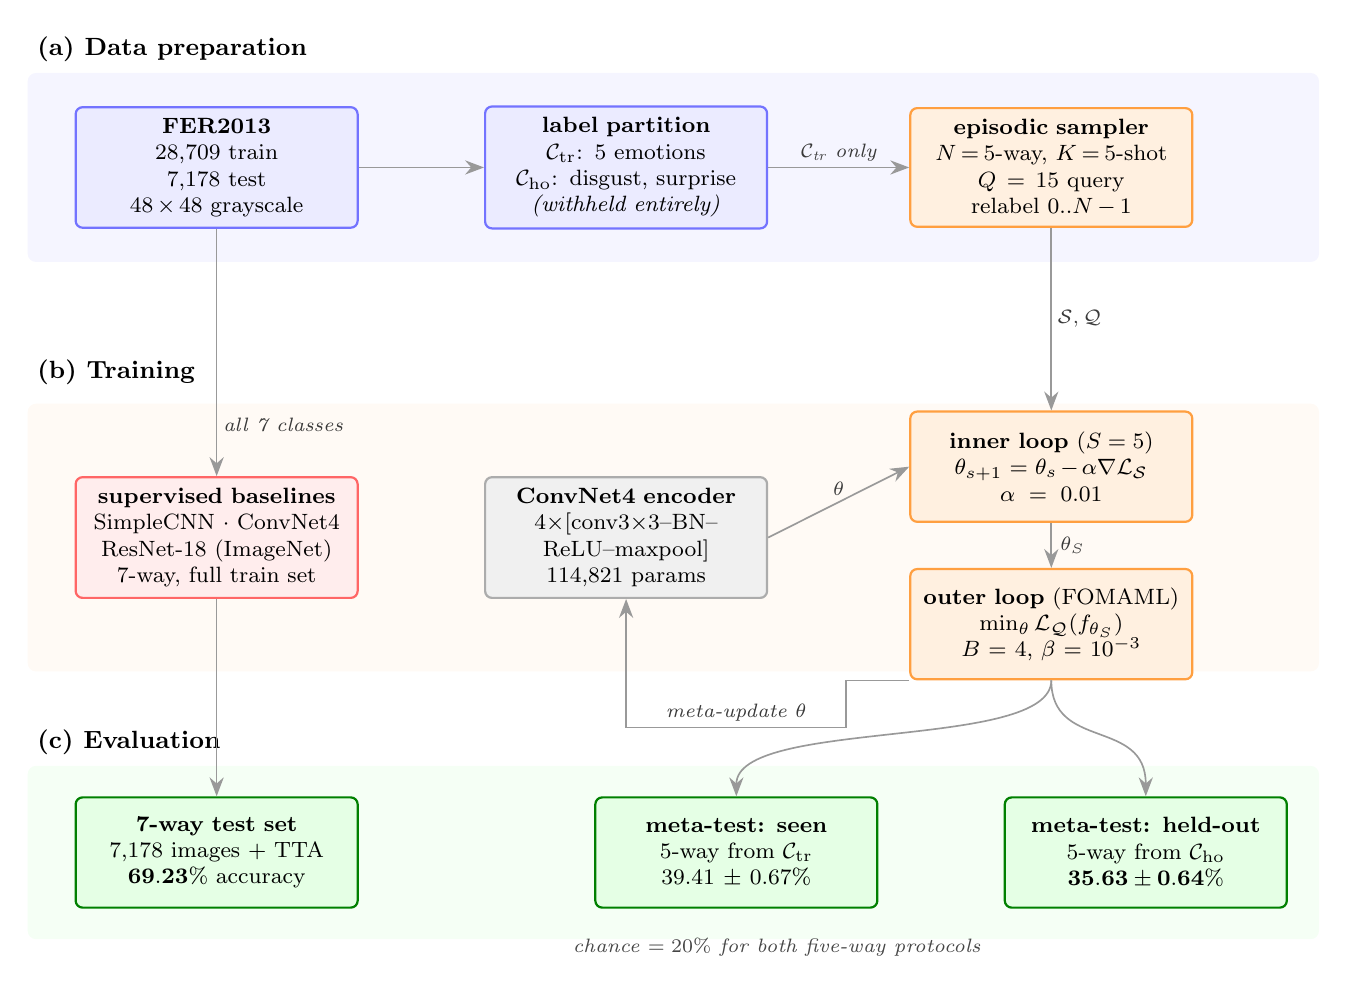
\begin{tikzpicture}[
  font=\footnotesize,
  box/.style={draw,rounded corners=2.5pt,align=center,
              minimum height=14mm,text width=33mm,inner sep=4pt},
  data/.style={box,fill=blue!8,draw=blue!55,thick},
  proc/.style={box,fill=orange!12,draw=orange!75,thick},
  enc/.style={box,fill=gray!12,draw=gray!65,thick},
  eval/.style={box,fill=green!10,draw=green!50!black,thick},
  base/.style={box,fill=red!7,draw=red!60,thick},
  ar/.style={-{Stealth[length=2.4mm,width=1.8mm]},semithick,draw=gray!80},
  lbl/.style={font=\scriptsize\itshape,text=gray!45!black,inner sep=2pt},
  stage/.style={font=\small\bfseries,anchor=west},
  sub/.style={font=\scriptsize\itshape,text=gray!55!black,anchor=west}
]

%%%%%%%%%%%%%%%%%%%%%% background bands per stage %%%%%%%%%%%%%%%%%%%%%%%%%
\begin{scope}[on background layer]
  \fill[rounded corners=3pt,blue!4]   (-2mm, 12mm) rectangle (162mm,-12mm);
  \fill[rounded corners=3pt,orange!4] (-2mm,-30mm) rectangle (162mm,-64mm);
  \fill[rounded corners=3pt,green!4]  (-2mm,-76mm) rectangle (162mm,-98mm);
\end{scope}

%%%%%%%%%%%%%%%%%%%%%% (a) DATA PREPARATION %%%%%%%%%%%%%%%%%%%%%%%%%%%%%%%
\node[stage] at (-2mm, 15mm) {(a) Data preparation};
\node[data] (fer)   at ( 22mm,0) {\textbf{FER2013}\\$28{,}709$ train\\$7{,}178$ test\\$48\!\times\!48$ grayscale};
\node[data] (split) at ( 74mm,0) {\textbf{label partition}\\$\mathcal{C}_{\text{tr}}$: 5 emotions\\$\mathcal{C}_{\text{ho}}$: disgust, surprise\\\emph{(withheld entirely)}};
\node[proc] (samp)  at (128mm,0) {\textbf{episodic sampler}\\$N\!=\!5$-way, $K\!=\!5$-shot\\$Q\!=\!15$ query\\relabel $0..N\!-\!1$};

\draw[ar] (fer)   -- (split);
\draw[ar] (split) -- node[lbl,above]{$\mathcal{C}_{\text{tr}}$ only} (samp);

%%%%%%%%%%%%%%%%%%%%%% (b) TRAINING %%%%%%%%%%%%%%%%%%%%%%%%%%%%%%%%%%%%%%%
\node[stage] at (-2mm,-26mm) {(b) Training};
\node[base] (sup)   at ( 22mm,-47mm) {\textbf{supervised baselines}\\SimpleCNN $\cdot$ ConvNet4\\ResNet-18 (ImageNet)\\7-way, full train set};
\node[enc]  (encod) at ( 74mm,-47mm) {\textbf{ConvNet4 encoder}\\$4\times$[conv$3{\times}3$--BN--\\ReLU--maxpool]\\$114{,}821$ params};
\node[proc] (inner) at (128mm,-38mm) {\textbf{inner loop} ($S\!=\!5$)\\$\theta_{s+1}\!=\!\theta_s\!-\!\alpha\nabla\mathcal{L}_{\mathcal{S}}$\\$\alpha\!=\!0.01$};
\node[proc] (outer) at (128mm,-58mm) {\textbf{outer loop} (FOMAML)\\$\min_\theta\mathcal{L}_{\mathcal{Q}}(f_{\theta_S})$\\$B\!=\!4$, $\beta\!=\!10^{-3}$};

\draw[ar] (fer.south) -- node[lbl,right,pos=0.80]{all 7 classes} (sup.north);
\draw[ar] (samp.south) -- node[lbl,right]{$\mathcal{S},\mathcal{Q}$} (inner.north);
\draw[ar] (encod.east) -- node[lbl,above]{$\theta$} (inner.west);
\draw[ar] (inner.south) -- node[lbl,right,inner sep=3pt]{$\theta_S$} (outer.north);
\draw[ar] (outer.south west) -- ++(-8mm,0) -- ++(0,-6mm) -|
      node[lbl,above,pos=0.25]{meta-update $\theta$} (encod.south);

%%%%%%%%%%%%%%%%%%%%%% (c) EVALUATION %%%%%%%%%%%%%%%%%%%%%%%%%%%%%%%%%%%%%
\node[stage] at (-2mm,-73mm) {(c) Evaluation};
\node[eval] (ev3) at ( 22mm,-87mm) {\textbf{7-way test set}\\$7{,}178$ images $+$ TTA\\$\mathbf{69.23\%}$ accuracy};
\node[eval] (ev1) at ( 88mm,-87mm) {\textbf{meta-test: seen}\\5-way from $\mathcal{C}_{\text{tr}}$\\$39.41 \pm 0.67\%$};
\node[eval] (ev2) at (140mm,-87mm) {\textbf{meta-test: held-out}\\5-way from $\mathcal{C}_{\text{ho}}$\\$\mathbf{35.63 \pm 0.64\%}$};

\draw[ar] (sup.south)   -- (ev3.north);
\draw[ar] (outer.south) .. controls +(0,-9mm) and +(0,10mm) .. (ev1.north);
\draw[ar] (outer.south) .. controls +(0,-9mm) and +(0,10mm) .. (ev2.north);

\node[sub] at (66mm,-99mm) {chance $=20\%$ for both five-way protocols};
\end{tikzpicture}%
}
\caption{\textbf{System overview.} \emph{(a)} The label set is partitioned
\emph{before} any training: five emotions are available to the meta-learner,
while \emph{disgust} and \emph{surprise} are withheld entirely. The episodic
sampler draws $N$-way $K$-shot tasks with within-episode relabelling.
\emph{(b)} Two training branches share the same source data. The supervised
baselines solve the conventional seven-way problem; the meta-learning branch
adapts a copy of the encoder parameters to each episode's support set (inner
loop) and updates the initialisation $\theta$ so that the adapted parameters
minimise query loss (outer loop). \emph{(c)} Evaluation under three protocols.
The held-out protocol, rightmost, is the central claim of this report:
episodes composed of emotions the meta-learner never observed.}
\label{fig:pipeline}
\end{figure}

\subsection{Network architectures}
The meta-learner uses \textbf{ConvNet4}, the four-block encoder standard in the
few-shot literature~\cite{vinyals2016matching,finn2017model}: four repetitions
of $3\times3$ convolution ($64$ channels), batch normalisation, ReLU and
$2\times2$ max-pooling, followed by a linear head, totalling $114{,}821$
parameters.

Batch normalisation uses batch statistics rather than running averages
(\texttt{track\_\-running\_\-stats=False}). This is a deliberate choice: episodic
training presents a different class distribution in every task, so running
estimates accumulated across tasks would leak information between episodes and
undermine the validity of the few-shot evaluation.

The strongest baseline is an ImageNet-pretrained
\textbf{ResNet-18}~\cite{he2016deep} ($11{,}173{,}831$ parameters). Two
adaptations are required.

\begin{enumerate}\itemsep3pt
\item \textbf{Resolution.} Inputs are bilinearly upsampled $48 \to 224$ on
device, so that the pretrained filters operate at the spatial scale for which
they were learned. Feeding $48\times48$ directly wastes the pretraining, and
this is the single most consequential design decision in this report.

\item \textbf{Channel count.} The RGB stem is collapsed to one channel by
summing the first convolution's weights across the input dimension,
$W'_{o,1,i,j} = \sum_{c=1}^{3} W_{o,c,i,j}$. This preserves each filter's
response to grayscale structure at one third of the stem compute relative to
replicating the input three times.
\end{enumerate}

\subsection{Dataset and preprocessing}
\label{sec:data}
FER2013 provides $28{,}709$ training and $7{,}178$ test images across the seven
classes. Table~\ref{tab:dataset} gives the per-class composition; the
$16.5{:}1$ ratio between \emph{happiness} and \emph{disgust} is the central
difficulty the method addresses.

\begin{table}[htbp]
\centering
\small
\begin{tabular}{lrrr}
\toprule
Emotion & Train & Test & Share of train \\
\midrule
Anger      & $3{,}995$  & $958$     & $13.9\%$ \\
Disgust    & $436$      & $111$     & $1.5\%$ \\
Fear       & $4{,}097$  & $1{,}024$ & $14.3\%$ \\
Happiness  & $7{,}215$  & $1{,}774$ & $25.1\%$ \\
Neutral    & $4{,}965$  & $1{,}233$ & $17.3\%$ \\
Sadness    & $4{,}830$  & $1{,}247$ & $16.8\%$ \\
Surprise   & $3{,}171$  & $831$     & $11.0\%$ \\
\midrule
\textbf{Total} & $\mathbf{28{,}709}$ & $\mathbf{7{,}178}$ & $100\%$ \\
\bottomrule
\end{tabular}
\caption{FER2013 composition. The imbalance ratio between the most and least
frequent training classes is $16.5{:}1$.}
\label{tab:dataset}
\end{table}

Twenty percent of the training split is held out for validation, stratified by
class so that the validation distribution matches training. Images are scaled
to $[0,1]$ and normalised by statistics computed over the training split only
($\mu = 0.5077$, $\sigma = 0.2550$), so that evaluation never sees test
statistics.

Augmentation is applied to training data only and comprises horizontal flipping
(faces are near-symmetric, so the operation is label-preserving), rotation
$\pm15^\circ$ and scaling $[0.9,1.1]$ applied as a single affine warp about the
image centre, translation up to $10\%$, and random
erasing~\cite{zhong2020random} of a patch with probability $0.25$.

\paragraph{A defect worth reporting.}
Translation is frequently implemented with \texttt{np.roll}, which is
\emph{circular}: pixels shifted off one edge reappear on the opposite edge, so
a translated face acquires a strip of its own opposite side. The resulting
images cannot occur in any real camera and teach the model edge artefacts. This
was a defect in the first implementation used here, and it appears in published
code. Translation is now performed with zero fill.

\subsection{Implementation and training configuration}
All experiments use PyTorch on a single NVIDIA RTX 3050 Laptop GPU ($4$\,GB)
with an Intel i7-11800H CPU. The GPU thermally throttles to approximately
$22\%$ of its rated clock under sustained load, which affects reported
wall-clock times but not the results themselves. Table~\ref{tab:hyper} lists
the settings.

\begin{table}[htbp]
\centering
\small
\begin{tabular}{lll}
\toprule
& \textbf{Meta-learning (MAML)} & \textbf{Supervised baselines} \\
\midrule
Optimiser        & Adam (outer loop)         & AdamW \\
Learning rate    & $\beta = 10^{-3}$         & $10^{-3}$ / $3\times10^{-4}$ (ResNet) \\
Inner step size  & $\alpha = 0.01$           & --- \\
Inner steps      & $S = 5$                   & --- \\
Task batch       & $B = 4$                   & --- \\
Batch size       & ---                       & $128$ / $64$ (ResNet-18) \\
Duration         & $2{,}000$ meta-iterations & up to $150$ epochs \\
Schedule         & constant                  & cosine annealing \\
Weight decay     & ---                       & $10^{-4}$ \\
Label smoothing  & ---                       & $\varepsilon = 0.05$ \\
Gradient clip    & norm $10$                 & --- \\
Evaluation       & $300$ episodes, $95\%$ CI & full test set $+$ TTA \\
\bottomrule
\end{tabular}
\caption{Training configuration. All values are fixed before a run and recorded
alongside its results.}
\label{tab:hyper}
\end{table}

Batch size $64$ at $224\times224$ is the largest that fits in $4$\,GB (peak
allocation $1.50$\,GB, measured). Test-time augmentation averages softmax
outputs over the image and its horizontal flip.

\paragraph{Checkpoint selection.}
Under label smoothing on noisy labels, validation loss and accuracy can move in
opposite directions: a model that becomes more accurate while also more
confident is penalised by cross-entropy. Because the criterion governs both
checkpointing and early stopping, it is exposed as an explicit setting
(\texttt{-{}-monitor}) fixed before a run begins and recorded with the results.
Both choices are reported in Section~\ref{sec:ablation} rather than one being
selected after inspecting the curves.

%%%%%%%%%%%%%%%%%%%%%%%%%%%%%%%%%%%%%%%%%%%%%%%%%%%%%%%%%%%%%%%%%%%%%%%%%%%%
\section{Results}
\label{sec:results}

\subsection{Supervised baselines}
Table~\ref{tab:baselines} reports the seven-way comparison. Because of the
$16.5{:}1$ imbalance, balanced accuracy and macro-F1 are reported alongside raw
accuracy; plain accuracy rewards a model that concentrates on frequent classes.

\begin{table}[htbp]
\centering
\small
\begin{tabular}{lrrrrr}
\toprule
Model & Params & Accuracy & Balanced acc. & Macro-F1 & Train (min) \\
\midrule
SimpleCNN                     & $1.27$M & $42.89$ & $37.20$ & $33.98$ & $3.9$ \\
ConvNet4 ($30$ ep.)           & $0.12$M & $49.61$ & $50.83$ & $46.38$ & $5.4$ \\
ConvNet4 tuned                & $0.45$M & $50.93$ & $52.11$ & $47.53$ & $39.4$ \\
ResNet-18 (loss-ckpt)         & $11.2$M & $66.93$ & $65.57$ & $62.48$ & $49.8$ \\
\textbf{ResNet-18 (acc-ckpt)} & $11.2$M & $\mathbf{69.23}$ & $\mathbf{68.18}$ & $\mathbf{66.29}$ & $100.8$ \\
\midrule
\multicolumn{6}{l}{\emph{Published reference points}} \\
Human ceiling~\cite{goodfellow2013challenges} & --- & ${\sim}65$ & --- & --- & --- \\
Kaggle 2013 winner~\cite{tang2013deep}        & --- & $71.2$     & --- & --- & --- \\
State of the art~\cite{khaireddin2021facial}  & --- & $73$--$76$ & --- & --- & --- \\
\bottomrule
\end{tabular}
\caption{\textbf{Supervised baselines} on the seven-way FER2013 test set, all
values percentages. The strongest model exceeds the estimated human ceiling and
sits $1.97$ points below the score that won the original competition.}
\label{tab:baselines}
\end{table}

Two observations follow. First, the $0.12$M-parameter ConvNet4 outperforms the
$1.27$M-parameter SimpleCNN by $6.7$ accuracy points and by $12.4$ points on
macro-F1. Capacity is not the binding constraint at this scale; architecture
is.

Second, extending ConvNet4 from $30$ to $150$ epochs with stronger augmentation
and a wider backbone bought only $1.3$ points ($49.61 \to 50.93$) at eight
times the compute, and the run early-stopped at epoch $76$ with a $20$-point
train--validation gap. This is reported as a negative result: scratch-trained
models of this size saturate well below the dataset ceiling, and the jump to
$69.23\%$ comes from ImageNet pretraining rather than from longer schedules.

\subsection{Checkpoint selection ablation}
\label{sec:ablation}
Table~\ref{tab:ckpt} isolates the criterion. Both runs share architecture,
seed, data order, optimiser and schedule; only the monitored quantity differs,
and it was declared before training in each case.

\begin{table}[htbp]
\centering
\small
\begin{tabular}{lrrrrr}
\toprule
Criterion & Epochs run & Best epoch & Accuracy & Balanced acc. & Macro-F1 \\
\midrule
Validation loss     & $18$ & $10$ & $66.93$ & $65.57$ & $62.48$ \\
Validation accuracy & $30$ & $27$ & $\mathbf{69.23}$ & $\mathbf{68.18}$ & $\mathbf{66.29}$ \\
\midrule
\emph{Difference} & & & $+2.30$ & $+2.61$ & $+3.81$ \\
\bottomrule
\end{tabular}
\caption{\textbf{Checkpoint selection under label smoothing.} Selecting by
validation loss both retains worse weights and halts training $12$ epochs
early, while validation accuracy was still improving.}
\label{tab:ckpt}
\end{table}

The mechanism is clear. Validation loss reached its minimum at epoch $10$ and
rose thereafter, while validation accuracy continued to improve until epoch
$27$. Loss-based early stopping therefore terminated the run at epoch $18$ on a
model that was still improving by the metric of interest. The gain is largest
on macro-F1 ($+3.81$), concentrated in the hardest classes: \emph{fear}
improves by $9.2$ F1 points and \emph{disgust} by $7.3$.

\subsection{Per-class analysis}
Table~\ref{tab:perclass} compares the best scratch-trained model against the
best pretrained one.

\begin{table}[htbp]
\centering
\small
\begin{tabular}{lrrrrrrr}
\toprule
& & \multicolumn{3}{c}{ConvNet4 tuned} & \multicolumn{3}{c}{ResNet-18 (acc-ckpt)}\\
\cmidrule(lr){3-5}\cmidrule(lr){6-8}
Emotion & $n$ & Prec. & Rec. & F1 & Prec. & Rec. & F1 \\
\midrule
Anger     & $958$     & $45.9$ & $41.9$ & $43.8$ & $61.4$ & $64.8$ & $63.1$ \\
Disgust   & $111$     & $26.8$ & $73.9$ & $39.3$ & $47.8$ & $69.4$ & $56.6$ \\
Fear      & $1{,}024$ & $37.2$ & $31.3$ & $34.0$ & $57.8$ & $48.0$ & $52.5$ \\
Happiness & $1{,}774$ & $75.9$ & $72.3$ & $74.0$ & $90.4$ & $86.5$ & $88.4$ \\
Neutral   & $1{,}233$ & $41.8$ & $56.4$ & $48.0$ & $63.2$ & $67.6$ & $65.3$ \\
Sadness   & $1{,}247$ & $42.1$ & $32.3$ & $36.6$ & $57.5$ & $57.7$ & $57.6$ \\
Surprise  & $831$     & $57.2$ & $56.7$ & $56.9$ & $78.0$ & $83.2$ & $80.5$ \\
\bottomrule
\end{tabular}
\caption{\textbf{Per-class test performance}, percentages. \emph{Disgust}
illustrates why precision must be read alongside recall: ConvNet4 attains
$73.9\%$ recall at only $26.8\%$ precision, over-predicting the rare class
because of the class weighting, whereas ResNet-18 reaches $47.8\%$ precision at
comparable recall.}
\label{tab:perclass}
\end{table}

\emph{Fear} remains the hardest category for both models, consistent with the
literature. At $48\times48$ it is genuinely confusable with \emph{surprise} and
\emph{sadness}, and a substantial share of the residual error is attributable
to label noise rather than to model capacity.

\subsection{Few-shot results}
Table~\ref{tab:maml} reports meta-test accuracy under both protocols.

\begin{table}[htbp]
\centering
\small
\begin{tabular}{lrrrr}
\toprule
Protocol & Chance & Accuracy ($95\%$ CI) & $\times$ chance & Episodes \\
\midrule
Seen emotions ($\mathcal{C}_{\text{tr}}$)     & $20.0$ & $39.41 \pm 0.67$ & $1.97$ & $300$ \\
\textbf{Held-out} ($\mathcal{C}_{\text{ho}}$) & $20.0$ & $\mathbf{35.63 \pm 0.64}$ & $1.78$ & $300$ \\
\bottomrule
\end{tabular}
\caption{\textbf{Five-way five-shot meta-test accuracy}, mean over $300$
episodes with $95\%$ confidence intervals. The held-out protocol uses
\emph{disgust} and \emph{surprise}, excluded from meta-training entirely.}
\label{tab:maml}
\end{table}

From five labelled examples per class, the meta-learned initialisation reaches
$35.63\%$ on emotions it never observed during training --- $15.6$ points above
chance, and within $3.8$ points of its own performance on seen emotions.

The narrow gap between the two protocols is the substantive finding of this
report. It indicates that the initialisation encodes features transferable
across affective categories rather than a representation specialised to the
training emotions. Had the model merely memorised the five meta-training
classes, held-out performance would have collapsed toward chance; it does not.

\paragraph{On comparing the two settings.}
The few-shot figures are five-way ($20\%$ chance) and the supervised figures
seven-way ($14.3\%$ chance), measured on different label sets. They answer
different questions and are deliberately not placed in a single table:
$69.23\%$ supervised and $35.63\%$ few-shot are not commensurable, and treating
them as such would misrepresent both.

\subsection{Summary of ablations}
\begin{itemize}\itemsep3pt
\item \textbf{ImageNet pretraining}: $50.93 \to 69.23$, $+18.3$ points. By far
the largest single factor.
\item \textbf{Checkpoint criterion} (Table~\ref{tab:ckpt}): $+2.30$ accuracy,
$+3.81$ macro-F1.
\item \textbf{Test-time augmentation}: $68.47 \to 69.23$, $+0.76$ accuracy, at
negligible cost.
\item \textbf{Schedule length} (ConvNet4, $30 \to 150$ epochs with stronger
augmentation and doubled width): $+1.32$ only, with an early stop at epoch
$76$. Reported as a negative result; it is what identified architecture rather
than schedule as the binding constraint.
\end{itemize}

%%%%%%%%%%%%%%%%%%%%%%%%%%%%%%%%%%%%%%%%%%%%%%%%%%%%%%%%%%%%%%%%%%%%%%%%%%%%
\section{Conclusion}
\label{sec:conclusion}

This report studied facial emotion recognition under the constraint that
matters in deployment: that the emotions of greatest interest are those with
the least data. Casting the problem episodically and meta-learning an
initialisation with first-order MAML produced $35.63 \pm 0.64\%$ five-way
accuracy on emotions withheld entirely from meta-training, from five labelled
examples per class against a $20\%$ chance level. Alongside this, a calibrated
supervised reference reaching $69.23\%$ seven-way accuracy was established,
above the estimated human ceiling for this dataset.

\paragraph{Restated contributions.}
The held-out-emotion protocol is a materially stronger test than the
conventional few-shot evaluation, and the small measured gap between seen and
unseen emotions ($3.8$ points) is evidence that the learned initialisation is
not merely memorising training categories. Separately, the checkpoint-selection
ablation shows that a default many practitioners never revisit --- monitoring
validation loss --- costs $2.30$ accuracy points when label smoothing is
combined with noisy labels.

\paragraph{Significance.}
The practical implication is that a deployed FER system need not wait for a
balanced corpus before supporting a new affective category. A handful of
labelled examples recovers most of the performance the same architecture
achieves on categories it was trained on, which changes the economics of
extending such a system.

\paragraph{Limitations.}
Several constraints bound these conclusions. Evaluation is confined to FER2013,
whose $48\times48$ grayscale images and noisy labels cap achievable accuracy at
roughly $73$--$76\%$; results may not transfer to higher-resolution corpora
such as AffectNet or RAF\nobreakdash-DB. The held-out set contains only two emotions, so
the unseen-category estimate rests on a narrow base. The first-order MAML
approximation was used throughout for memory reasons and the second-order
variant was not measured. All runs used a single seed, so no variance across
initialisations is reported. Finally, the supervised model remains $4$--$7$
points below published state of the art, which relies on ensembling and
auxiliary pretraining data that the available hardware could not accommodate.

\paragraph{Future work.}
The natural extensions are a larger held-out set via leave-one-emotion-out
cross-validation; pretraining on AffectNet before meta-training, to separate
representation quality from meta-learning; comparison against metric-based
few-shot methods~\cite{snell2017prototypical}; and multi-seed runs to quantify
variance.

%%%%%%%%%%%%%%%%%%%%%%%%%%%%%%%%%%%%%%%%%%%%%%%%%%%%%%%%%%%%%%%%%%%%%%%%%%%%
\section{Contributions}
\label{sec:contributions}

The division of work between the two authors is set out below. It is uneven,
and is reported as it occurred.

\vspace{0.25cm}
\noindent
\textbf{MD AL Amin} (Matricola VR510263)

\begin{itemize}\itemsep2pt
\item \textbf{Coding.} The complete implementation: the data pipeline and
episodic sampler (\texttt{data.py}), including the stratified train/validation
split and the augmentation policy; the network architectures
(\texttt{models.py}), comprising SimpleCNN, ConvNet4 and its functional forward
pass; the meta-learning core (\texttt{maml.py}), comprising the inner
adaptation loop, the first-order meta-update and the episodic evaluation
routine; the three training entry points (\texttt{train\_maml.py},
\texttt{train\_baseline.py}, \texttt{train\_pretrained.py}); the evaluation and
figure-generation code (\texttt{evaluate.py}); and the supporting scripts.

\item \textbf{Experiments.} All six training runs: SimpleCNN; ConvNet4 at
$30$ epochs; ConvNet4 tuned at $150$ epochs; MAML $5$-way $5$-shot; and the two
ResNet-18 runs under loss- and accuracy-based checkpointing. This includes the
checkpoint-selection ablation of Section~\ref{sec:ablation} and the per-class
analysis of Section~\ref{sec:results}.

\item \textbf{Writing.} The Method section (Section~\ref{sec:method}),
including the formal treatment of MAML and the description of the
architectures and training configuration, and the Results section
(Section~\ref{sec:results}), including the interpretation of the baseline
comparison and the few-shot protocols.
\end{itemize}

\vspace{0.25cm}
\noindent
\textbf{Md.\ Nazibul Islam} (Matricola VR528950)

\begin{itemize}\itemsep2pt
\item \textbf{Literature review.} The survey underpinning
Section~\ref{sec:intro}: the FER2013 benchmark and its published results, from
the original competition through to current state of the art; the few-shot
learning literature, covering both optimisation-based and metric-based
approaches; and the augmentation literature. This review established the gap
the report addresses, namely that existing few-shot evaluations of FER sample
episodes from the training emotion set and therefore measure adaptation to
unseen images rather than to unseen categories.

\item \textbf{Figures.} Preparation of the figures and tables presenting the
experimental results, including the confusion matrices, the training curves and
the system overview diagram (Figure~\ref{fig:pipeline}).

\item \textbf{Manuscript review.} Review of the full manuscript for technical
accuracy and consistency of the reported figures across sections.
\end{itemize}

\vspace{0.25cm}
\noindent
The framing of the problem, the design of the held-out-emotion protocol and the
choice of \emph{disgust} and \emph{surprise} as the withheld classes emerged
from joint discussion between both authors, as did the decision to adopt
first-order MAML. Both authors reviewed and approved the final manuscript.

%%%%%%%%%%%%%%%%%%%%%%%%%%%%%%%%%%%%%%%%%%%%%%%%%%%%%%%%%%%%%%%%%%%%%%%%%%%%
\newpage
\begin{thebibliography}{99}
\small

\bibitem{goodfellow2013challenges}
I.~J. Goodfellow, D.~Erhan, P.~L. Carrier, A.~Courville, M.~Mirza, et~al.
\newblock Challenges in representation learning: A report on three machine
  learning contests.
\newblock In {\em International Conference on Neural Information Processing
  (ICONIP)}, 2013.

\bibitem{tang2013deep}
Y.~Tang.
\newblock Deep learning using linear support vector machines.
\newblock In {\em ICML Workshop on Representation Learning}, 2013.

\bibitem{finn2017model}
C.~Finn, P.~Abbeel, and S.~Levine.
\newblock Model-agnostic meta-learning for fast adaptation of deep networks.
\newblock In {\em International Conference on Machine Learning (ICML)}, 2017.

\bibitem{nichol2018first}
A.~Nichol, J.~Achiam, and J.~Schulman.
\newblock On first-order meta-learning algorithms.
\newblock {\em arXiv preprint arXiv:1803.02999}, 2018.

\bibitem{snell2017prototypical}
J.~Snell, K.~Swersky, and R.~Zemel.
\newblock Prototypical networks for few-shot learning.
\newblock In {\em Advances in Neural Information Processing Systems
  (NeurIPS)}, 2017.

\bibitem{vinyals2016matching}
O.~Vinyals, C.~Blundell, T.~Lillicrap, K.~Kavukcuoglu, and D.~Wierstra.
\newblock Matching networks for one shot learning.
\newblock In {\em Advances in Neural Information Processing Systems
  (NeurIPS)}, 2016.

\bibitem{he2016deep}
K.~He, X.~Zhang, S.~Ren, and J.~Sun.
\newblock Deep residual learning for image recognition.
\newblock In {\em IEEE Conference on Computer Vision and Pattern Recognition
  (CVPR)}, 2016.

\bibitem{khaireddin2021facial}
Y.~Khaireddin and Z.~Chen.
\newblock Facial emotion recognition: State of the art performance on FER2013.
\newblock {\em arXiv preprint arXiv:2105.03588}, 2021.

\bibitem{pramerdorfer2016facial}
C.~Pramerdorfer and M.~Kampel.
\newblock Facial expression recognition using convolutional neural networks:
  State of the art.
\newblock {\em arXiv preprint arXiv:1612.02903}, 2016.

\bibitem{zhong2020random}
Z.~Zhong, L.~Zheng, G.~Kang, S.~Li, and Y.~Yang.
\newblock Random erasing data augmentation.
\newblock In {\em AAAI Conference on Artificial Intelligence}, 2020.

\end{thebibliography}

\end{document}
